\documentclass{article}
\usepackage[utf8]{inputenc}
\usepackage{amsmath,listings}
\usepackage{multicol}
\usepackage{tikz}
\usetikzlibrary{arrows.meta, positioning}

\title{Parallax Technical Specifications}
\author{Draft v0.1}
\date{\today}

\begin{document}

\maketitle

\section{Introduction}
This document is the primary reference for the Parallax programming language. It officially describes the language constructs. \textit{This document is currently in draft stage and is constantly evolving.}

\section{Goals}
We want to design a high-level programming language that allows easy instruction-level parallelism for its users. It is designed to be efficient and look elegant. We aim for predictive low-level performance and control over SIMD primitives in modern processors. The target architectures include AVX512 and amd64 for vector and scalar instructions, respectively.

\section{Lexical Structure}

\subsection{Notations}
The syntax of the language is given in extended BNF notation.

\subsection{Encoding}
All Parallax source files are in UTF-8 encoding. Other encodings are not supported. The line termination sequences can be Unix (LF), Windows (CR LF), or Macintosh (CR).

\subsection{Blanks and Comments}
Blanks include spaces, tabs, and form feeds. They are ignored unless separating identifiers. Comments start with `\#' and run until the end of the line.

\begin{verbatim}
i = 0     # This is a comment
\end{verbatim}

Documentation comments start with two `\#' symbols and are part of the syntax tree.

\section{Identifiers and Keywords}
Identifiers are any string of letters, digits, and underscores but must begin with a letter and cannot end with an underscore. Case sensitivity is ignored.





\[
\text{letter} ::= 'A' \dots 'Z' \mid 'a' \dots 'z'
\]

\[
\text{digit} ::= '0' \dots '9'
\]

\[
\text{hex} ::= [-] \ (0x) \ ( \text{digit} \mid 'A' \dots 'F' \mid 'a' \dots 'f' )
\]

\[
\text{octal} ::= [-] \ (0o) \ ( '0' \dots '7' )
\]

\[
\text{binary} ::= [-] \ (0b) \ ( '0' \dots '1' )
\]

\[
\text{decimal} ::= ( '1' \dots '9' ) \ \text{digit}^*
\]

\[
\text{INTEGER} ::= [-] \ \text{decimal} \mid \text{hex-integer} \mid \text{octal}
\]

\[
\text{FLOAT} ::= [-] \ ( \text{decimal} \ [ . \ \text{digit} ] )
\]

\[
\text{IDENTIFIER} ::= \text{letter} \ ( ['\_'] ( \text{letter} \mid \text{digit} ) )^*
\]




\noindent \textbf{Reserved Keywords:}

\vspace{10pt}
\begin{center}
\begin{tabular}{ l l l }
\texttt{and}   & \texttt{break}     & \texttt{const}     \\
\texttt{continue}  & \texttt{comptime} & \texttt{else}      \\
\texttt{enum}   & \texttt{except}   & \texttt{export}   \\
\texttt{for}    & \texttt{fn}        & \texttt{if}        \\
\texttt{import}  & \texttt{in}      & \texttt{macro}    \\
\texttt{mut}    & \texttt{not}      & \texttt{or}       \\
\texttt{return} & \texttt{static}   & \texttt{while}     \\
\end{tabular}
\end{center}

\section{Types}
Parallax is a strongly-typed static language. All types are immutable by default. The \texttt{mut} keyword declares an identifier as mutable.

\[
\texttt{type\_t [mut] identifier = expression}
\]

\subsection{Primitive Types}

We currently support the following primitive types:

\begin{multicols}{2}
    \begin{itemize}
        \item \texttt{u8}, \texttt{u16}, \texttt{u32}, \texttt{u64}
        \item \texttt{i8}, \texttt{i16}, \texttt{i32}, \texttt{i64}
        \item \texttt{f32}, \texttt{f64}
        \item \texttt{tensor<>} (more complex, harder to implement than vector/array)
    \end{itemize}
\end{multicols}

\subsubsection{Vectorized Types}

We also support vectorized types for SIMD (Single Instruction, Multiple Data) operations. These include:

\begin{lstlisting}[basicstyle=\ttfamily]
u.x1, u.x2, u.x4, u.x8, u.x16, u.x32, u.x64
i.x1, i.x2, i.x4, i.x8, i.x16, i.x32, i.x64
f.x1, f.x2, f.x4, f.x8, f.x16, f.x32, f.x64
\end{lstlisting}

Where \texttt{xN} indicates the number of elements in the vector. For example:
\begin{itemize}
    \item \texttt{u16x16} corresponds to a 256-bit SIMD register (YMM for x86, V register for ARM).
    \item \texttt{u16x1} can either be padded or fit along with other values, depending on the implementation (could fit into scalar registers such as \texttt{rax}).
\end{itemize}

\subsection{Character and String Types}

\subsubsection{Character Type (\texttt{char})}

A \texttt{char} is defined by the following grammar:

\[
\texttt{char} \rightarrow ' (' \mid \backslash i \mid \texttt{space} \mid \backslash (\texttt{[a-zA-Z]} \mid \texttt{ascii} \mid \texttt{decimal})) '
\]

\subsubsection{String Type (\texttt{string})}

A \texttt{string} is defined as:

\[
\texttt{string} \rightarrow \texttt{"} \{ \backslash i \mid \texttt{space} \mid (\texttt{[a-zA-Z]} \mid \texttt{ascii} \mid \texttt{decimal} \mid \texttt{gap}) \} \texttt{"}
\]

\subsection{SIMD Registers for Vectorized Types}

For SIMD operations, different registers are used based on the type and architecture:
\begin{itemize}
    \item \textbf{XMM Register}: 128-bit wide, used for x86 SIMD instructions.
    \item \textbf{YMM Register}: 256-bit wide, also for x86 SIMD (YMM is an extension of XMM).
    \item \textbf{V Register}: 128-bit wide, used for ARM SIMD operations.
\end{itemize}

\subsection{No Pointer/Reference Types}

Parallax does not have explicit pointer or reference types. Internally, all variables, objects, and functions are passed by reference. This behavior might be extended later with something akin to Rust’s \texttt{clone()} to explicitly pass by value.

\subsection{User-defined Structs}

Users can define their own structs to group and organize data.

\section{Operators and Expressions}
Unary and binary operators follow a precedence order. Statements end with semicolons.


\section{Grammar Rules}

\subsection{Translation Unit}
\[
\langle \text{translation-unit} \rangle ::= \{ \langle \text{external-declaration} \rangle \}^*
\]

\subsection{External Declaration}
\[
\langle \text{external-declaration} \rangle ::= \langle \text{function-definition} \rangle 
\mid \langle \text{declaration} \rangle
\]

\subsection{Function Definition}
\[
\langle \text{function-definition} \rangle ::= \texttt{fn} \ \langle \text{IDENTIFIER} \rangle \ ( \{ \langle \text{parameter} \rangle \}^* ) \ \{ \{ \langle \text{statement} \rangle \}^* \}
\]

\subsection{Declaration}
\[
\langle \text{declaration} \rangle ::= \langle \text{declaration-specifier} \rangle \ \langle \text{declarator} \rangle \ ;
\]

\subsection{Declaration Specifier}
\[
\langle \text{declaration-specifier} \rangle ::= \langle \text{type-specifier} \rangle
\]

\subsection{Type Specifier}
\[
\langle \text{type-specifier} \rangle ::= \texttt{u8} \mid \texttt{u16} \mid \texttt{u32} \mid \texttt{u64} 
\mid \texttt{i8} \mid \texttt{i16} \mid \texttt{i32} \mid \texttt{i64} 
\mid \texttt{float} \mid \texttt{double}
\]

\subsection{Declarator}
\[
\langle \text{declarator} \rangle ::= \langle \text{IDENTIFIER} \rangle \mid * \langle \text{IDENTIFIER} \rangle
\]

\subsection{Statement}
\[
\langle \text{statement} \rangle ::= \langle \text{expression} \rangle \ ; 
\mid \langle \text{compound-statement} \rangle 
\mid \langle \text{declaration} \rangle 
\mid \langle \text{if-statement} \rangle 
\mid \langle \text{for-loop} \rangle 
\mid \langle \text{return-statement} \rangle
\]

\subsection{Compound Statement}
\[
\langle \text{compound-statement} \rangle ::= \{ \{ \langle \text{statement} \rangle \}^* \}
\]

\subsection{Expression}
\[
\langle \text{expression} \rangle ::= \langle \text{primary-expression} \rangle 
\mid \langle \text{expression} \rangle + \langle \text{expression} \rangle 
\mid \langle \text{expression} \rangle - \langle \text{expression} \rangle 
\mid \langle \text{expression} \rangle * \langle \text{expression} \rangle 
\mid \langle \text{expression} \rangle / \langle \text{expression} \rangle 
\mid \langle \text{assignment-expression} \rangle
\]

\subsection{Primary Expression}
\[
\langle \text{primary-expression} \rangle ::= \langle \text{IDENTIFIER} \rangle 
\mid \langle \text{constant} \rangle 
\mid ( \langle \text{expression} \rangle )
\]

\subsection{Assignment Expression}
\[
\langle \text{assignment-expression} \rangle ::= \langle \text{IDENTIFIER} \rangle = \langle \text{expression} \rangle
\]

\subsection{Parameter}
\[
\langle \text{parameter} \rangle ::= \langle \text{declaration-specifier} \rangle \ \langle \text{declarator} \rangle
\]

\subsection{If Statement}
\[
\langle \text{if-statement} \rangle ::= \texttt{if} ( \langle \text{expression} \rangle ) \langle \text{compound-statement} \rangle 
\mid \texttt{if} ( \langle \text{expression} \rangle ) \langle \text{compound-statement} \rangle \ \texttt{else} \ \langle \text{compound-statement} \rangle
\]

\subsection{For Loop}
\[
\langle \text{for-loop} \rangle ::= \texttt{for} ( \langle \text{declaration} \rangle \langle \text{expression} \rangle ; \langle \text{expression} \rangle ) \langle \text{compound-statement} \rangle
\]

\subsection{Return Statement}
\[
\langle \text{return-statement} \rangle ::= \texttt{return} \ \langle \text{expression} \rangle? \ ;
\]

\subsection{Constant}
\[
\langle \text{constant} \rangle ::= \langle \text{INTEGER} \rangle \mid \langle \text{FLOAT} \rangle
\]

\subsection{Integer}
\[
\langle \text{INTEGER} \rangle ::= [-]? \langle \text{decimal} \rangle 
\mid [-]? \langle \text{hex} \rangle 
\mid [-]? \langle \text{octal} \rangle 
\mid [-]? \langle \text{binary} \rangle
\]

\subsection{Float}
\[
\langle \text{FLOAT} \rangle ::= [-]? \langle \text{decimal} \rangle [ "." \langle \text{digit} \rangle^*]
\]

\subsection{Decimal}
\[
\langle \text{decimal} \rangle ::= ( '1' \dots '9' ) \langle \text{digit} \rangle^*
\]

\subsection{Hexadecimal}
\[
\langle \text{hex} \rangle ::= \texttt{0x} \langle \text{digit} \rangle \mid 'A' \dots 'F' \mid 'a' \dots 'f'
\]

\subsection{Octal}
\[
\langle \text{octal} \rangle ::= \texttt{0o} '0' \dots '7'
\]

\subsection{Binary}
\[
\langle \text{binary} \rangle ::= \texttt{0b} '0' \dots '1'
\]
\subsection{Identifier}
\[
\langle \text{IDENTIFIER} \rangle ::= \langle \text{letter} \rangle \, ( \texttt{['\_']} \, ( \langle \text{letter} \rangle \mid \langle \text{digit} \rangle ) )^*
\]

\subsection{Letter}
\[
\langle \text{letter} \rangle ::= 'A' \dots 'Z' \mid 'a' \dots 'z'
\]

\subsection{Digit}
\[
\langle \text{digit} \rangle ::= '0' \dots '9'
\]

\subsection{String Literal}
\[
\langle \text{string-literal} \rangle ::= " \langle \text{character} \rangle^* "
\]


\subsection{String}
\[
\langle \text{STRING} \rangle ::= \langle \text{string-literal} \rangle
\]

\subsection{Abstract Syntax Tree}
 
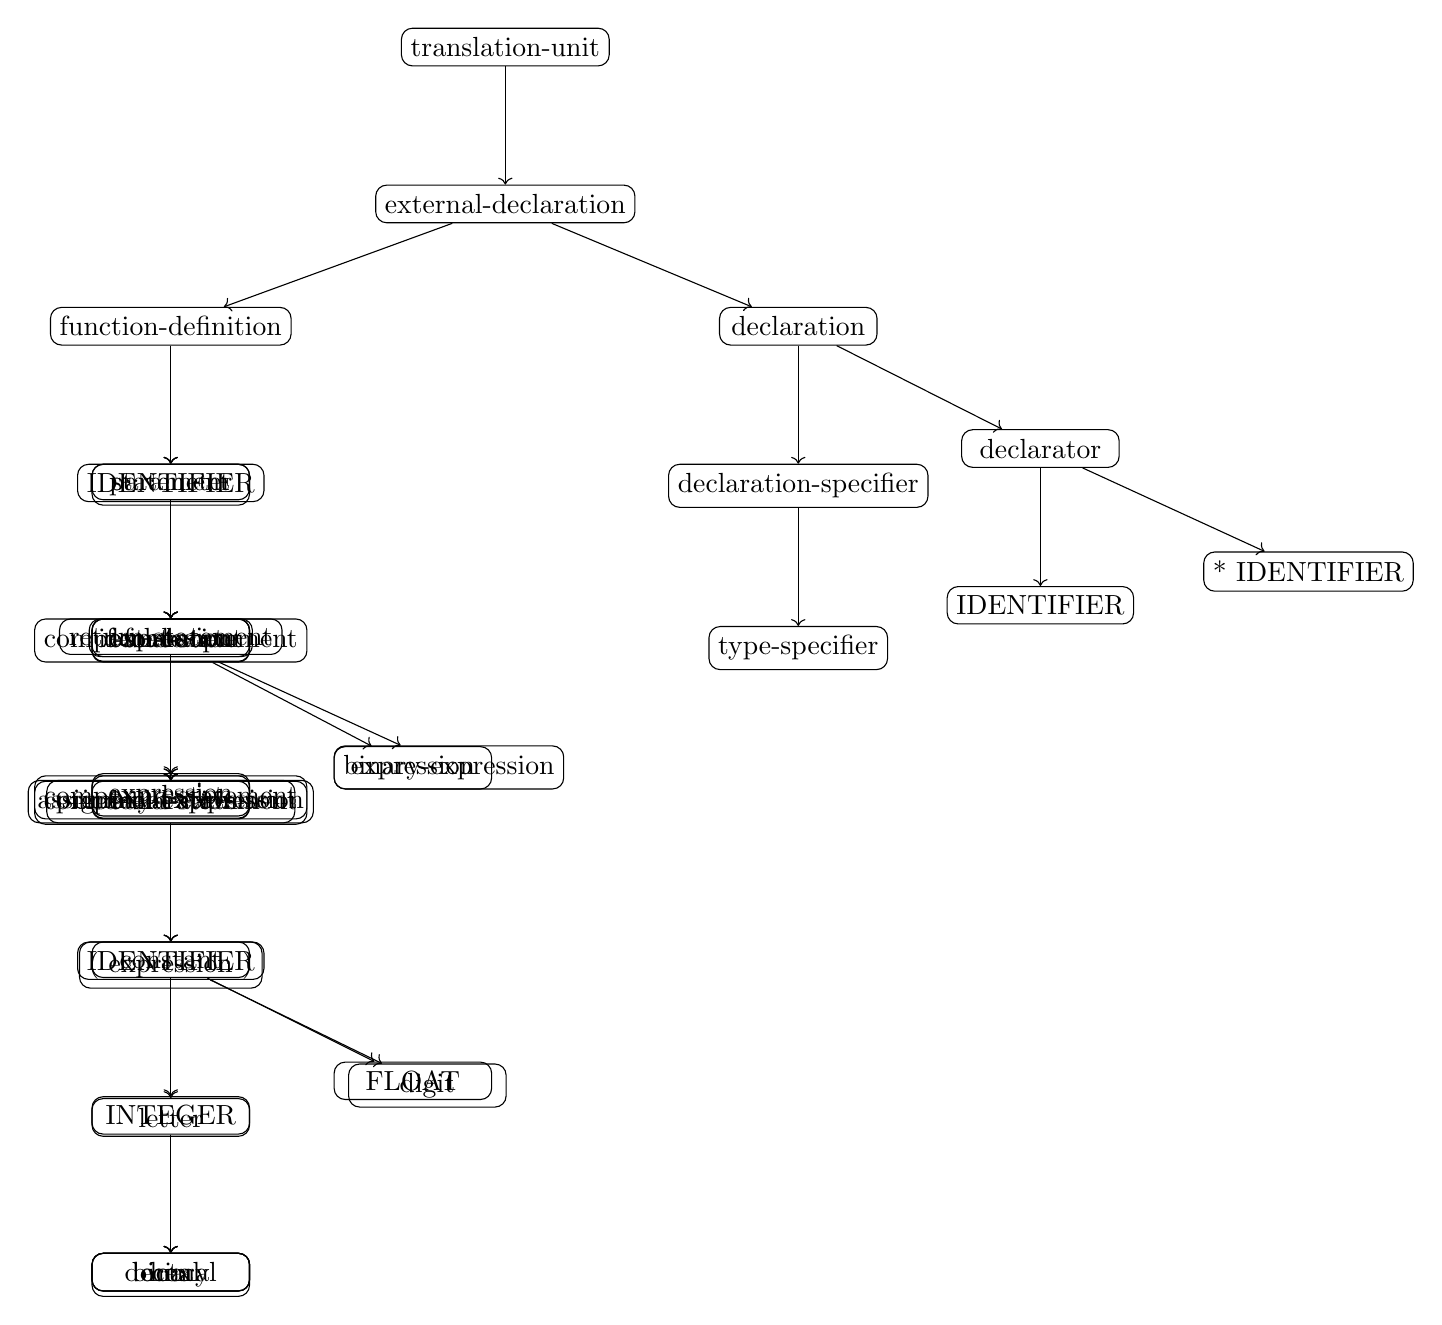
\begin{tikzpicture}[
    node distance=1.5cm,
    every node/.style={draw, rounded corners, align=center, minimum width=2cm},
    ->, % Default arrow tip
]
    % Nodes
    \node (A) {translation-unit};
    \node (B) [below=of A] {external-declaration};
    \node (C) [below left=of B] {function-definition};
    \node (D) [below right=of B] {declaration};
    
    \node (E) [below=of C] {IDENTIFIER};
    \node (F) [below=of C] {parameter};
    \node (G) [below=of C] {statement};
    
    \node (H) [below=of D] {declaration-specifier};
    \node (I) [below right=of D] {declarator};
    
    \node (J) [below=of H] {type-specifier};
    
    \node (K) [below=of I] {IDENTIFIER};
    \node (L) [below right=of I] {* IDENTIFIER};
    
    \node (M) [below=of G] {expression};
    \node (N) [below=of G] {compound-statement};
    \node (O) [below=of G] {declaration};
    \node (P) [below=of G] {if-statement};
    \node (Q) [below=of G] {for-loop};
    \node (R) [below=of G] {return-statement};
    
    \node (S) [below=of M] {primary-expression};
    \node (T) [below right=of M] {binary-expression};
    \node (U) [below=of M] {assignment-expression};
    
    \node (V) [below=of S] {IDENTIFIER};
    \node (W) [below=of S] {constant};
    \node (X) [below=of S] {( expression )};
    
    \node (Y) [below=of W] {INTEGER};
    \node (Z) [below right=of W] {FLOAT};
    
    \node (AA) [below=of Y] {decimal};
    \node (AB) [below=of Y] {hex};
    \node (AC) [below=of Y] {octal};
    \node (AD) [below=of Y] {binary};
    
    \node (AE) [below=of V] {letter};
    \node (AF) [below right=of V] {digit};
    
    \node (AG) [below=of P] {expression};
    \node (AH) [below=of P] {compound-statement};
    
    \node (AI) [below=of Q] {declaration};
    \node (AJ) [below right=of Q] {expression};
    \node (AK) [below=of Q] {compound-statement};
    
    \node (AL) [below=of R] {expression};
    
    % Connections
    \draw (A) -- (B);
    \draw (B) -- (C);
    \draw (B) -- (D);
    
    \draw (C) -- (E);
    \draw (C) -- (F);
    \draw (C) -- (G);
    
    \draw (D) -- (H);
    \draw (D) -- (I);
    
    \draw (H) -- (J);
    
    \draw (I) -- (K);
    \draw (I) -- (L);
    
    \draw (G) -- (M);
    \draw (G) -- (N);
    \draw (G) -- (O);
    \draw (G) -- (P);
    \draw (G) -- (Q);
    \draw (G) -- (R);
    
    \draw (M) -- (S);
    \draw (M) -- (T);
    \draw (M) -- (U);
    
    \draw (S) -- (V);
    \draw (S) -- (W);
    \draw (S) -- (X);
    
    \draw (W) -- (Y);
    \draw (W) -- (Z);
    
    \draw (Y) -- (AA);
    \draw (Y) -- (AB);
    \draw (Y) -- (AC);
    \draw (Y) -- (AD);
    
    \draw (V) -- (AE);
    \draw (V) -- (AF);
    
    \draw (P) -- (AG);
    \draw (P) -- (AH);
    
    \draw (Q) -- (AI);
    \draw (Q) -- (AJ);
    \draw (Q) -- (AK);
    
    \draw (R) -- (AL);

\end{tikzpicture}


\section{Error Handling}
We are considering a \texttt{try/catch} mechanism, possibly similar to \texttt{Result} types in Rust. Null values may be avoided for performance reasons.

\section{Memory Management}
We are exploring garbage collection strategies and will investigate ownership and borrowing concepts.

\section{Optimizations}

\subsection{Constant Folding}
Constant folding evaluates constant expressions at compile time, reducing runtime computations by pre-calculating known values.

\subsection{Loop Unrolling}
Loop unrolling replicates the loop body multiple times to reduce loop overhead. This technique can improve instruction-level parallelism and cache utilization.

\subsection{Constant Propagation}
Constant propagation replaces variables with their constant values throughout the code. This enables further optimizations and simplifies computations.

\subsection{Dead Code Elimination}
Dead code elimination removes code that does not affect the program's output, improving performance and reducing code size.

\subsection{Function Inlining}
Function inlining replaces function calls with the function's body, reducing call overhead and enabling further optimizations.

\subsection{Instruction Scheduling}
Instruction scheduling reorders instructions to maximize pipeline efficiency, improving instruction-level parallelism and CPU utilization.

\subsection{Data Layout Optimization}
Data layout optimization reorganizes data structures to improve cache locality, enhancing memory access patterns and overall performance.

\subsection{Auto Vectorization}
Auto vectorization automatically converts scalar operations to vector operations, leveraging SIMD instructions for improved parallel processing. This is the major optimization we want to research.


\end{document}
